\documentclass[a4paper]{article}

\usepackage[utf8]{inputenc}


\title{\textbf{Práctica 3: Fundamentos de la ciencia de datos}}
\author{Luis Alejandro Cabanillas, Alvaro de las Heras, Mohssin Nagib Najim}

\usepackage{Sweave}
\begin{document}
\Sconcordance{concordance:practica-3.tex:practica-3.Rnw:%
1 8 1 1 0 28 1 1 3 1 0 2 1 12 0 1 3 3 1 1 2 16 0 1 2 1 1 1 2 4 0 1 2 1 %
1 1 2 16 0 1 2 5 1 1 2 14 0 1 2 11 1 1 2 11 0 1 2 1 1 1 2 4 0 1 2 1 1 1 %
2 1 0 1 1 3 0 1 2 1 1 1 -3 1 8 24 1 1 3 1 0 2 1 12 0 1 3 2 1 1 3 20 0 1 %
3 1 2 17 0 1 2 3 1 1 2 18 0 1 2 1 1 1 2 16 0 1 2 3 1 1 2 51 0 1 2 1 1 1 %
2 1 0 2 1 16 0 2 1 16 0 2 1 16 0 2 1 17 0 1 2 2 1 1 2 11 0 1 1 10 0 1 1 %
10 0 1 1 11 0 1 2 2 1 1 2 1 0 8 1 3 0 1 2 1 -2 1 7 5 1 1 2 7 0 1 2 3 1 %
1 2 7 0 1 2 3 1 1 2 7 0 1 2 3 1 1 2 7 0 1 2 10 1 1 2 1 0 5 1 3 0 1 2 1 %
5 4 0 5 1 29 0 1 2 3 1 1 3 2 0 2 1 22 0 2 2 1 0 1 1 4 0 1 2 1 1 1 3 2 0 %
2 1 22 0 1 2 1 4 7 0 1 2 4 1 1 4 6 0 1 2 2 1 1 2 5 0 1 2 2 1 1 4 6 0 2 %
2 5 0 1 2 2 1 1 4 6 0 2 2 5 0 1 2 2 1 1 3 2 0 1 1 12 0 1 1 19 0 1 2 2 1 %
1 3 5 0 2 2 1 0 1 1 4 0 1 2 8 1 1 2 1 0 1 2 1 0 4 1 1 3 5 0 2 2 5 0 1 2 %
4 1 1 2 1 0 1 1 53 0 1 2 2 1 1 2 5 0 1 2 8 1 1 4 18 0 1 1 15 0 1 2 7 0 %
1 1 6 0 1 1 6 0 1 2 13 0 2 1 7 0 1 2 2 1}



\maketitle

\section{Ejercicio 1}La primera parte de la práctica consistirá en la realización de dos ejercicios de clasificación de datos con R, aplicando todos los conocimientos vistos en clase.

Los datos en este ejercicio serán relativos a las calificaciones de un grupo de alumnos en teoría, laboratorio y prácticas, respectivamente. La última nota es la calificación global, que en este caso será el clasificador. Contamos con la siguiente muestra:
\begin{itemize}
	\item \textbf{{A, A, B, Ap}}
	\item \textbf{{A, B, D, Ss}}
	\item \textbf{{D, D, C, Ss}}
        \item \textbf{{D, D, A, Ss}}
        \item \textbf{{B, C, B, Ss}}
        \item \textbf{{C, B, B, Ap}}
        \item \textbf{{B, B, A, Ap}}
        \item \textbf{{C, D, C, Ss}}
        \item \textbf{{B, A, C, Ss}}
\end{itemize}

\subsection{Árboles de decisión de Hunt} Lo primero que tendremos que hacer es descargar los paquetes tree y rpart, que utilizaremos para ejecutar el algoritmo de clasificación elegido sobre la muestra de datos. Para ello ejecutaremos:

\begin{itemize}
	\item \textbf{{install.packages("rpart")}}
	\item \textbf{{install.packages("tree")}}
\end{itemize}

Una vez descargados, los cargaremos en el entorno actual con library:
\begin{Schunk}
\begin{Sinput}
> library("rpart")
> library("tree")
> search()
\end{Sinput}
\begin{Soutput}
 [1] ".GlobalEnv"        "package:tree"      "package:rpart"    
 [4] "package:foreign"   "package:stats"     "package:graphics" 
 [7] "package:grDevices" "package:utils"     "package:datasets" 
[10] "package:methods"   "Autoloads"         "package:base"     
\end{Soutput}
\begin{Sinput}
> 
\end{Sinput}
\end{Schunk}

Como podemos ver, tras ejecutar search, tenemos los paquetes cargados y listos para utilizarse.

Lo siguiente que tendremos que hacer es introducir la muestra de datos en un archivo .txt y leer este archivo con R:
\begin{Schunk}
\begin{Sinput}
> (calificaciones<-read.table("notas.txt"))
\end{Sinput}
\begin{Soutput}
        Teoria Lab Pract C.Globl
suceso1      A   A     B      Ap
suceso2      A   B     D      Ss
suceso3      D   D     C      Ss
suceso4      D   D     A      Ss
suceso5      B   C     B      Ss
suceso6      C   B     B      Ap
suceso7      B   B     A      Ap
suceso8      C   D     C      Ss
suceso9      B   A     C      Ss
\end{Soutput}
\end{Schunk}

Para poder ejecutar rpart sobre los datos de la muestra debemos convertir los datos leídos en un dataframe:
\begin{Schunk}
\begin{Sinput}
> muestra<-data.frame(calificaciones)
\end{Sinput}
\end{Schunk}

Ahora ya tenemos todo preparado para poder ejecutar el algoritmo sobre los datos.En los argumentos pondremos "C.Globl~." para inidicar cual es el clasificador (C.Globl~) y el punto para coger todos los datos de la muestra. Como segundo argumento le indicaremos a la función que los datos residen en la variable muestra y como método le indicaremos class. No hace falta que le indiquemos que queremos calcular las ganancias de información mediante gini ya que, como se indica en la página 21 del manual de rpart, el algortimo aplica gini por defecto. Así:
\begin{Schunk}
\begin{Sinput}
> (clasificacion=rpart(C.Globl~.,data=muestra, method="class", minsplit=1))
\end{Sinput}
\begin{Soutput}
n= 9 

node), split, n, loss, yval, (yprob)
      * denotes terminal node

1) root 9 3 Ss (0.3333333 0.6666667)  
  2) Lab=A,B 5 2 Ap (0.6000000 0.4000000)  
    4) Pract=A,B 3 0 Ap (1.0000000 0.0000000) *
    5) Pract=C,D 2 0 Ss (0.0000000 1.0000000) *
  3) Lab=C,D 4 0 Ss (0.0000000 1.0000000) *
\end{Soutput}
\end{Schunk}

Podemos observar que el algoritmo ha llevado a cabo la clasificación. En el nodo raíz tenemos Laboratorio , si en la nota de laboratorio el alumno tiene una C o una D, podemos saber que ha suspendido. Si tiene una A o una B hay que evaluar la nota de Prácticas. Si en práticas tienen una A o una B ha aprobado, en caso contrario (C o D) ha suspendido.

Así, el algoritmo de clasificación ha supuesto una ventaja, ya que no tenemos que evaluar la nota de Teoría para saber si el alumno ha aprobado o suspendido.

También podemos utilizar la función tree para obtener el árbol de clasificación, aunque da fallos con muestras de datos tan pequeñas.
\begin{Schunk}
\begin{Sinput}
> (clasificacionTree = tree(C.Globl~.,data=muestra, mincut=1,minsize=2))
\end{Sinput}
\begin{Soutput}
node), split, n, deviance, yval, (yprob)
      * denotes terminal node

1) root 9 11.46 Ss ( 0.3333 0.6667 )  
  2) Lab: A,B 5  6.73 Ap ( 0.6000 0.4000 )  
    4) Pract: A,B 3  0.00 Ap ( 1.0000 0.0000 ) *
    5) Pract: C,D 2  0.00 Ss ( 0.0000 1.0000 ) *
  3) Lab: C,D 4  0.00 Ss ( 0.0000 1.0000 ) *
\end{Soutput}
\end{Schunk}

Se puede apreciar que el árbol generado por rpart y tree es el mismo.

\subsection{Análisis de regresión lineal}En el segundo apartado de la práctica vamos a realizar un análisis de regresión lineal sobre los radios y densidades de cuatro planetas del sistema solar. De esta forma, la muestra está conformada por:
\begin{itemize}
	\item \textbf{{Mercurio, 2.4, 5.4}}
	\item \textbf{{Venus, 6.1, 5.2}}
	\item \textbf{{Tierra, 6.4, 5.5}}
        \item \textbf{{Marte, 3.4, 3.9}}
\end{itemize}

Estos datos los tendremos nuevamente en un .txt al que hemos llamado planetas. El primer paso es leer este txt:
\begin{Schunk}
\begin{Sinput}
> (planetas<-read.table("planetas.txt"))
\end{Sinput}
\begin{Soutput}
           R   D
Mercurio 2.4 5.4
Venus    6.1 5.2
Tierra   6.4 5.5
Marte    3.4 3.9
\end{Soutput}
\end{Schunk}

Una vez tenemos los datos en R, debemos generar la recta de regresión. La ecuación de una recta es \textbf{y=a+bx}. En nuestro caso, la y será la densidad y la x el radio. únicamente sabiendo esto ya podemos generar la recta de regresión, gracias a la función \textbf{lm}; que sirve para ajustar models lineales en R:
\begin{Schunk}
\begin{Sinput}
> regresion = lm(D~R,data=planetas)
\end{Sinput}
\end{Schunk}

Ahora deberemos mostrar esos datos gráficamente:
\begin{Schunk}
\begin{Sinput}
> plot(planetas)
> abline(regresion, col="blue")
\end{Sinput}
\end{Schunk}

\begin{center}
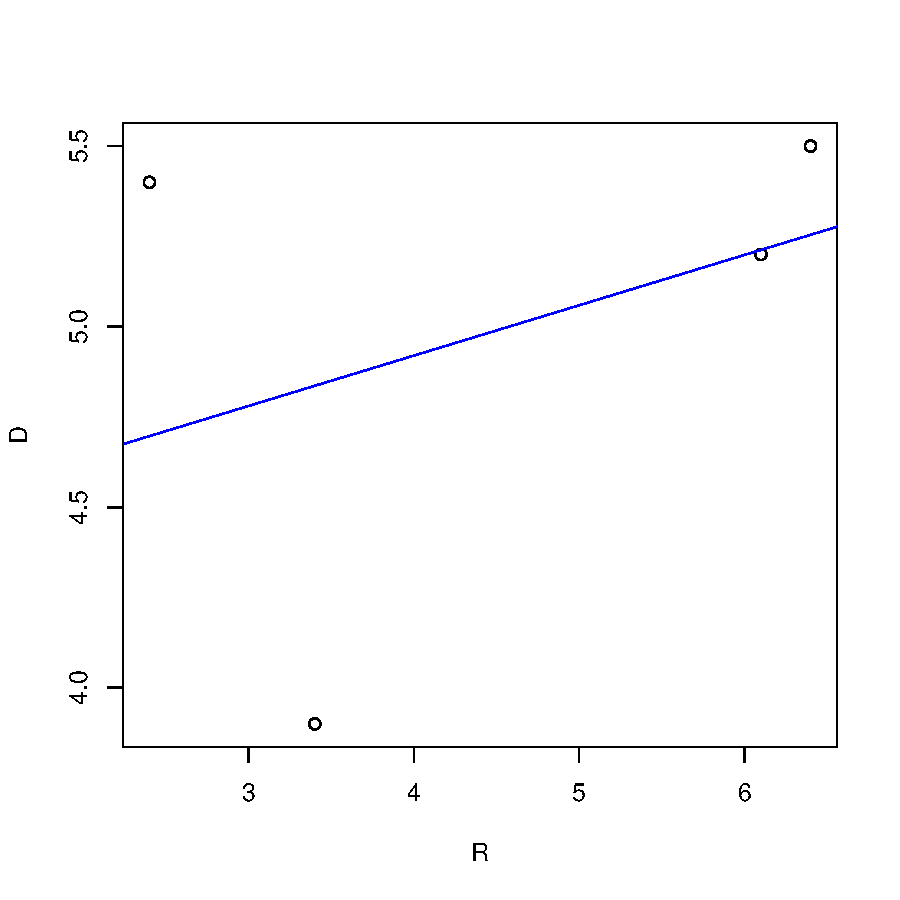
\includegraphics{practica-3-009}
\end{center}

Como podemos ver en la gráfica, la recta separa los datos correctamente.
\section{Ejercicio 2} En la segunda parte de la práctica se nos propone un realizar un análisis
de una muestra proporcionada en el mismo formada por las características de 10 vehiculos de cuatro
tipos diferentes. Con cuatro datos por vehiculo {TipoCarnet, NumeroRuedas, NumeroPasajeros, TipoVehiculo}.

La muestra que hemos obtenido consta de 10 características:
\begin{itemize}
	\item \textbf{{B, 4, 5, Coche}}
	\item \textbf{{A, 2, 2, Moto}}
	\item \textbf{{N, 2, 1, Bicicleta}}
        \item \textbf{{B, 6, 4, Camión}}
        \item \textbf{{B, 4, 6, Coche}}
        \item \textbf{{B, 4, 4, Coche}}
        \item \textbf{{N, 2, 2, Bicicleta}}
        \item \textbf{{B, 2, 1, Moto}}
        \item \textbf{{B, 6, 2, Camión}}
        \item \textbf{{N, 2, 1, Bicicleta}}

\end{itemize}

\subsection{Instalación paquete}
Para la realización de este ejercicio necesitaremos los paquetes, "rpart" y "tree" previamente instalados en el anterior ejercicio:

\begin{Schunk}
\begin{Sinput}
> library("rpart")
> library("tree")
> search()
\end{Sinput}
\begin{Soutput}
 [1] ".GlobalEnv"        "package:tree"      "package:rpart"    
 [4] "package:foreign"   "package:stats"     "package:graphics" 
 [7] "package:grDevices" "package:utils"     "package:datasets" 
[10] "package:methods"   "Autoloads"         "package:base"     
\end{Soutput}
\begin{Sinput}
> 
\end{Sinput}
\end{Schunk}

\subsection{Introducción de los datos de la muestra en R}
Los datos de las características de los coches los introduciremos en R por medio de un archivo .txt por lo que ejecutaremos los siguientes comandos:
\begin{Schunk}
\begin{Sinput}
> (vehiculos <- read.table("vehiculos.txt"))
\end{Sinput}
\begin{Soutput}
         TipoCarnet NumeroRuedas NumeroPasajeros TipoVehiculo
suceso1           B            4               5        Coche
suceso2           A            2               2         Moto
suceso3           N            2               1    Bicicleta
suceso4           B            6               4       Camion
suceso5           B            4               6        Coche
suceso6           B            4               4        Coche
suceso7           N            2               2    Bicicleta
suceso8           B            2               1         Moto
suceso9           B            6               2       Camion
suceso10          N            2               1    Bicicleta
\end{Soutput}
\begin{Sinput}
> 
\end{Sinput}
\end{Schunk}
El siguiente paso ser? convertirlo a data frame para poder trabajar con la muestra que tenemos:
\begin{Schunk}
\begin{Sinput}
> (muestraV = data.frame(vehiculos))
\end{Sinput}
\begin{Soutput}
         TipoCarnet NumeroRuedas NumeroPasajeros TipoVehiculo
suceso1           B            4               5        Coche
suceso2           A            2               2         Moto
suceso3           N            2               1    Bicicleta
suceso4           B            6               4       Camion
suceso5           B            4               6        Coche
suceso6           B            4               4        Coche
suceso7           N            2               2    Bicicleta
suceso8           B            2               1         Moto
suceso9           B            6               2       Camion
suceso10          N            2               1    Bicicleta
\end{Soutput}
\end{Schunk}

\subsection{Algoritmo de Hunt}
Utilizamos "rpart" para aplicar el algoritmo de Hunt utilizando la medida de la Ganancia de Información que trabaja con la medida
de impureza Gini por defecto y obtener la funci?n de clasificación (el árbol), como atributo clasificador utilizamos el tipo de vehiculo (TipoVehiculo):
\begin{Schunk}
\begin{Sinput}
> (clasificacionV = rpart(TipoVehiculo~., data=muestraV, method="class", minsplit=1))
\end{Sinput}
\begin{Soutput}
n= 10 

node), split, n, loss, yval, (yprob)
      * denotes terminal node

 1) root 10 7 Bicicleta (0.3000000 0.2000000 0.3000000 0.2000000)  
   2) TipoCarnet=N 3 0 Bicicleta (1.0000000 0.0000000 0.0000000 0.0000000) *
   3) TipoCarnet=A,B 7 4 Coche (0.0000000 0.2857143 0.4285714 0.2857143)  
     6) NumeroRuedas>=3 5 2 Coche (0.0000000 0.4000000 0.6000000 0.0000000)  
      12) NumeroRuedas>=5 2 0 Camion (0.0000000 1.0000000 0.0000000 0.0000000) *
      13) NumeroRuedas< 5 3 0 Coche (0.0000000 0.0000000 1.0000000 0.0000000) *
     7) NumeroRuedas< 3 2 0 Moto (0.0000000 0.0000000 0.0000000 1.0000000) *
\end{Soutput}
\end{Schunk}

También podemos utilizar la función tree para realizar el mismo proceso:
\begin{Schunk}
\begin{Sinput}
> (clasificaciontreeV = tree(TipoVehiculo~., data=muestraV, mincut=1, minsize=2))
\end{Sinput}
\begin{Soutput}
node), split, n, deviance, yval, (yprob)
      * denotes terminal node

1) root 10 27.32 Bicicleta ( 0.3 0.2 0.3 0.2 )  
  2) NumeroRuedas < 3 5  6.73 Bicicleta ( 0.6 0.0 0.0 0.4 )  
    4) TipoCarnet: A,B 2  0.00 Moto ( 0.0 0.0 0.0 1.0 ) *
    5) TipoCarnet: N 3  0.00 Bicicleta ( 1.0 0.0 0.0 0.0 ) *
  3) NumeroRuedas > 3 5  6.73 Coche ( 0.0 0.4 0.6 0.0 )  
    6) NumeroRuedas < 5 3  0.00 Coche ( 0.0 0.0 1.0 0.0 ) *
    7) NumeroRuedas > 5 2  0.00 Camion ( 0.0 1.0 0.0 0.0 ) *
\end{Soutput}
\end{Schunk}

Podemos ver los resultados al aplicar el algoritmo de optimización de Hunt que se nos genera el árbol final, el cual está estructurado en nodos y ramas.

\subsection{Análisis de regresión}En este segundo apartado tenemos que realizar un análisis de regresión sobre cuatro muestras de pares de datos situadas en un solo archivo .txt. El archivo que contiene las muestras se llamará muestra4.txt y tendrá todos los datos, especificados en el enunciado, en dos columnas:
\begin{Schunk}
\begin{Sinput}
> (muestra <- read.table("muestra4.txt"))
\end{Sinput}
\begin{Soutput}
    X     Y
1  10  8.04
2   8  6.95
3  13  7.58
4   9  8.81
5  11  8.33
6  14  9.96
7   6  7.24
8   4  4.26
9  12 10.84
10  7  4.82
11  5  5.68
12 10  9.14
13  8  8.14
14 13  8.74
15  9  8.77
16 11  9.26
17 14  8.10
18  6  6.13
19  4  3.10
20 12  9.13
21  7  7.26
22  5  4.74
23 10  7.46
24  8  6.77
25 13 12.74
26  9  7.11
27 11  7.81
28 14  8.84
29  6  6.08
30  4  5.39
31 12  8.15
32  7  6.42
33  5  5.73
34  8  6.58
35  8  5.76
36  8  7.71
37  8  8.84
38  8  8.47
39  8  7.04
40  8  5.25
41 19 12.50
42  8  5.56
43  8  7.91
44  8  6.89
\end{Soutput}
\end{Schunk}

Al tratarse de diferentes muestras, tenemos que dividir muestraDatos para obtener las cuatro muestras por separado y realizar el análisis de regresión sobre cada una de ellas. Para separar las muestras haremos uso de la función \textbf{split} de R, que sirve para dividir los datos de un vector en subgrupos:
\begin{Schunk}
\begin{Sinput}
> muestras <- split(muestra, factor(sort(rank(row.names(muestra))%%4)))
> muestra1 <- muestras[[1]]
> muestra1
\end{Sinput}
\begin{Soutput}
    X     Y
1  10  8.04
2   8  6.95
3  13  7.58
4   9  8.81
5  11  8.33
6  14  9.96
7   6  7.24
8   4  4.26
9  12 10.84
10  7  4.82
11  5  5.68
\end{Soutput}
\begin{Sinput}
> muestra2 <- muestras[[2]]
> muestra2
\end{Sinput}
\begin{Soutput}
    X    Y
12 10 9.14
13  8 8.14
14 13 8.74
15  9 8.77
16 11 9.26
17 14 8.10
18  6 6.13
19  4 3.10
20 12 9.13
21  7 7.26
22  5 4.74
\end{Soutput}
\begin{Sinput}
> muestra3 <- muestras[[3]]
> muestra3
\end{Sinput}
\begin{Soutput}
    X     Y
23 10  7.46
24  8  6.77
25 13 12.74
26  9  7.11
27 11  7.81
28 14  8.84
29  6  6.08
30  4  5.39
31 12  8.15
32  7  6.42
33  5  5.73
\end{Soutput}
\begin{Sinput}
> muestra4 <- muestras[[4]]
> muestra4
\end{Sinput}
\begin{Soutput}
    X     Y
34  8  6.58
35  8  5.76
36  8  7.71
37  8  8.84
38  8  8.47
39  8  7.04
40  8  5.25
41 19 12.50
42  8  5.56
43  8  7.91
44  8  6.89
\end{Soutput}
\end{Schunk}

Como podemos ver, ya tenemos los datos separados por muestras y podemos hacer el análisis de regresión sobre cada muestra:

\begin{Schunk}
\begin{Sinput}
> (regresion1 = lm(Y~X, data=muestra1))
\end{Sinput}
\begin{Soutput}
Call:
lm(formula = Y ~ X, data = muestra1)

Coefficients:
(Intercept)            X  
     3.0001       0.5001  
\end{Soutput}
\begin{Sinput}
> (regresion2 = lm(Y~X, data=muestra2))
\end{Sinput}
\begin{Soutput}
Call:
lm(formula = Y ~ X, data = muestra2)

Coefficients:
(Intercept)            X  
      3.001        0.500  
\end{Soutput}
\begin{Sinput}
> (regresion3 = lm(Y~X, data=muestra3))
\end{Sinput}
\begin{Soutput}
Call:
lm(formula = Y ~ X, data = muestra3)

Coefficients:
(Intercept)            X  
     3.0025       0.4997  
\end{Soutput}
\begin{Sinput}
> (regresion4 = lm(Y~X, data=muestra4))
\end{Sinput}
\begin{Soutput}
Call:
lm(formula = Y ~ X, data = muestra4)

Coefficients:
(Intercept)            X  
     3.0017       0.4999  
\end{Soutput}
\end{Schunk}

Por último, para visualizar las rectas de regresión en cada muestra de un vistazo hacemos uso de la función de R \textbf{par}, que nos permite consultar componentes gráficos. Le pasaremos como parámetro una matriz de 2x2 para que cada posición de esta sea ocupada por una gráfica:

\begin{Schunk}
\begin{Sinput}
> par(mfrow=c(2,2))
> plot(muestra1$X, muestra1$Y, main="Muestra 1", xlab="x", ylab="y")
> abline(regresion1, col="red")
> plot(muestra2$X, muestra2$Y, main="Muestra 2", xlab="x", ylab="y")
> abline(regresion2, col="blue")
> plot(muestra3$X, muestra3$Y, main="Muestra 3", xlab="x", ylab="y")
> abline(regresion3, col="green")
> plot(muestra4$X, muestra4$Y, main="Muestra 4", xlab="x", ylab="y")
> abline(regresion4, col="violet")
\end{Sinput}
\end{Schunk}

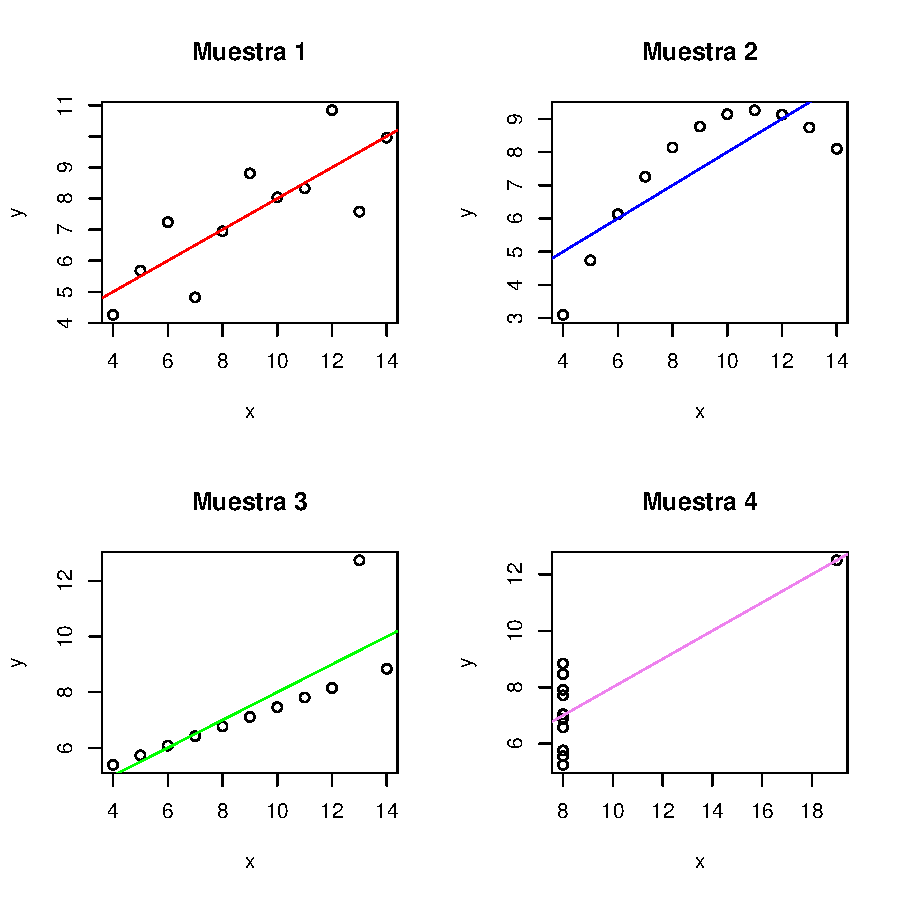
\includegraphics{practica-3-019}

Como podemos ver, hemos obtenido 4 gráficas con 4 rectas de regresión diferentes. Ahora vamos a estudiar la dependencia de los datos de cada muestra mediante la correlación.

\subsection{Correlación} Para calcular la correlación en R es tan fácil como usar la función \textbf{cor(variableX, variableY)}. Si la correlación tiene valor 1 o -1, la correlación es perfecta. En cambio, mientras más se acerque a 0, más débil será. Sabiendo esto vamos a estudiar el grado de correlación de cada muestra.

\subsubsection{Muestra 1} Para calcular la correlación en la muestra 1:
\begin{Schunk}
\begin{Sinput}
> cor(muestra1$X,muestra1$Y)
\end{Sinput}
\begin{Soutput}
[1] 0.8164205
\end{Soutput}
\end{Schunk}

Como podemos ver, la correlación tiene un valor cercano a 1, por lo que existe una correlación positiva fuerte.

\subsubsection{Muestra 2} Para calcular la correlación en la muestra 2:
\begin{Schunk}
\begin{Sinput}
> cor(muestra2$X,muestra2$Y)
\end{Sinput}
\begin{Soutput}
[1] 0.8162365
\end{Soutput}
\end{Schunk}

Nuevamente, la correlación tiene un valor cercano a 1, por lo que existe una correlación positiva fuerte.

\subsubsection{Muestra 3} Para calcular la correlación en la muestra 3:
\begin{Schunk}
\begin{Sinput}
> cor(muestra3$X,muestra3$Y)
\end{Sinput}
\begin{Soutput}
[1] 0.8162867
\end{Soutput}
\end{Schunk}

La correlación tiene un valor cercano a 1 y muy parecido a los dos anteriores, por lo que existe una correlación positiva fuerte.

\subsubsection{Muestra 4} Para calcular la correlación en la muestra 4:
\begin{Schunk}
\begin{Sinput}
> cor(muestra4$X,muestra4$Y)
\end{Sinput}
\begin{Soutput}
[1] 0.8165214
\end{Soutput}
\end{Schunk}

Como podemos ver, la correlación tiene un valor cercano a 1 y muy aproximado al resto de muestras, por lo que existe una correlación positiva fuerte en todas las muestras.

\section{Ejercicio 2}
\subsection{Ejercicio 2.3} 
En este ejercicio el objetivo será clasificar un conjunto de películas y valoraciones, este conjunto de datos lo hemos obtenido en Kaggle.com. 
La idea es realizar una serie de clasificaciones de diversos tipos, con varias técnicas, además de la visualización y prueba de estos mediante predicciones. Para necesitaremos las siguiente bibliotecas: 
\begin{itemize}
	\item \textbf{Visualización:} rpart.plot y ggplot2.
	\item \textbf{Clasificación:} rpart, tree, randomForest y BayesTree.
\end{itemize}
\begin{Schunk}
\begin{Sinput}
> library("rpart.plot")
> library("rpart")  
> library("tree")  
> library("ggplot2")
> library("randomForest") 
> library("BayesTree")  
\end{Sinput}
\end{Schunk}
Con las bibliotecas puestas el siguiente paso es cargar los datos, en este caso el archivo es un CSV, por lo que podemos leerlo directamente con R. Para optimizar la carga al leer seleccionamos las columnas que nos interesan ahorrando así cargar columnas que no son relevantes para el ejercicio, esto lo hacemos con el parámetro textbf{colClasses}. Una vez cargados los datos procederemos a limpiar los valores NA con textbf{na.omit(datos)}, para el problema definiremos distintos conjuntos de datos de 25, 1000 y todas las películas.
\begin{Schunk}
\begin{Sinput}
> columnas<-c("NULL","character","numeric","numeric","NULL","NULL",
+             "character","NULL","numeric","character","character",
+             "character","numeric", rep("NULL",6),"character","character",
+             "NULL","numeric","numeric","NULL","numeric","NULL","NULL")
> peliculas <- read.csv("imdb.csv",head=T,sep=",",encoding = "UTF-8",colClasses=columnas)
> peliculas<-na.omit(peliculas)
> pelis<-head(peliculas,25)
> mil_peliculas<-head(peliculas,1000)
> head(pelis,5)
\end{Sinput}
\begin{Soutput}
      director_name num_critic_for_reviews duration     actor_2_name     gross
1     James Cameron                    723      178 Joel David Moore 760505847
2    Gore Verbinski                    302      169    Orlando Bloom 309404152
3        Sam Mendes                    602      148     Rory Kinnear 200074175
4 Christopher Nolan                    813      164   Christian Bale 448130642
6    Andrew Stanton                    462      132  Samantha Morton  73058679
                           genres    actor_1_name
1 Action|Adventure|Fantasy|Sci-Fi     CCH Pounder
2        Action|Adventure|Fantasy     Johnny Depp
3       Action|Adventure|Thriller Christoph Waltz
4                 Action|Thriller       Tom Hardy
6         Action|Adventure|Sci-Fi    Daryl Sabara
                                movie_title num_voted_users language country
1                                   Avatar           886204  English     USA
2 Pirates of the Caribbean: At World's End           471220  English     USA
3                                  Spectre           275868  English      UK
4                    The Dark Knight Rises          1144337  English     USA
6                              John Carter           212204  English     USA
     budget title_year imdb_score
1 237000000       2009        7.9
2 300000000       2007        7.1
3 245000000       2015        6.8
4 250000000       2012        8.5
6 263700000       2012        6.6
\end{Soutput}
\end{Schunk}
A continuación aplicaremos los distintos métodos de clasificación para obtener datos
\subsubsection{Regresión lineal entre variables}
En esta sección se va estudiar la correlación entre distintas variables cuantitativas, para finalmente mostrar la recta de regresión que las define, para ello se realizarán distintos ejemplos.
En el primer caso vamos a comparar la relación que existe entre el número de votos y la puntuación de mil películas. En este caso si que existe una relación débil entre ambas variables, pero para este conjunto de datos es la mejor que se ha podido obtener, porque el valor de R cuadrado es de 0,40. La recta quedará definida por los coeficientes que se reflejan en el \textbf{summary()}, que son en este caso a = 5,897 y b =  3.164e-06. Además también tendrá una desviación del error de 0,762, que será la distancia entre lo predicho por la línea y los puntos reales.
\begin{Schunk}
\begin{Sinput}
> # Regresion entre votos y puntuacion
> comp<-data.frame(mil_peliculas["num_voted_users"],mil_peliculas["imdb_score"])
> reg.votos.imdb = lm(imdb_score~num_voted_users,data=mil_peliculas)
> summary(reg.votos.imdb)
\end{Sinput}
\begin{Soutput}
Call:
lm(formula = imdb_score ~ num_voted_users, data = mil_peliculas)

Residuals:
    Min      1Q  Median      3Q     Max 
-3.8263 -0.4154  0.0650  0.5344  1.8785 

Coefficients:
                 Estimate Std. Error t value Pr(>|t|)    
(Intercept)     5.897e+00  3.284e-02  179.60   <2e-16 ***
num_voted_users 3.164e-06  1.220e-07   25.93   <2e-16 ***
---
Signif. codes:  0 '***' 0.001 '**' 0.01 '*' 0.05 '.' 0.1 ' ' 1

Residual standard error: 0.7672 on 998 degrees of freedom
Multiple R-squared:  0.4026,	Adjusted R-squared:  0.402 
F-statistic: 672.5 on 1 and 998 DF,  p-value: < 2.2e-16
\end{Soutput}
\end{Schunk}

\begin{Schunk}
\begin{Sinput}
> plot(comp)
> abline(reg.votos.imdb, col="blue")
\end{Sinput}
\end{Schunk}
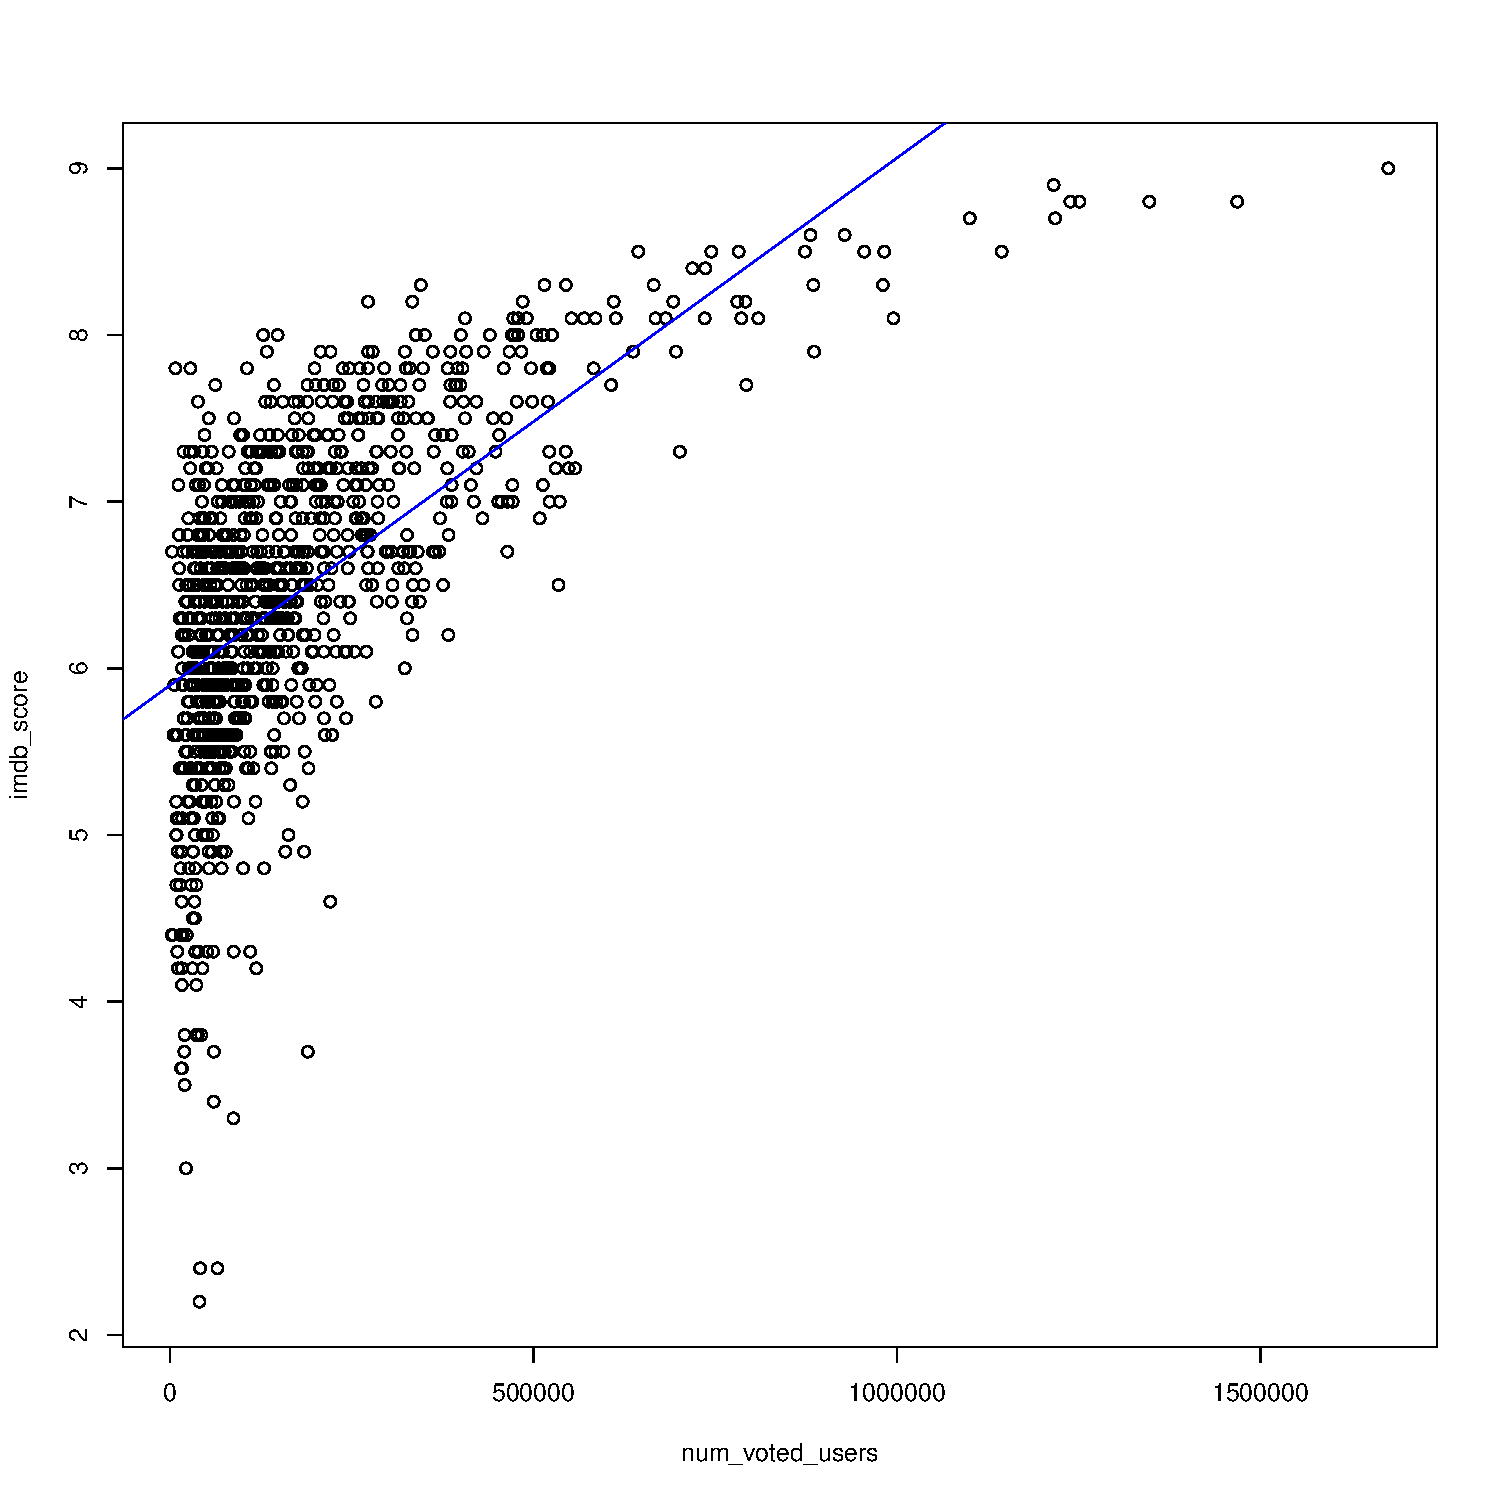
\includegraphics{practica-3-regresion1}

Estas variables se han elegido para comprobar como actua cuando no tiene apenas relación alguna las variables, como se observa en la gráfica se puede ver una nube de puntos cuya correlación es muy mala, como se ve con el R al cuadrado de 0,16, el error es mayor con 0,90 y los coeficientes son distintos.
\begin{Schunk}
\begin{Sinput}
> # Regresion entre duracion de una pelicula y puntuacion
> comp<-data.frame(mil_peliculas["duration"],mil_peliculas["imdb_score"])
> reg.duracion.imdb = lm(imdb_score~duration,data=mil_peliculas)
> summary(reg.duracion.imdb)
\end{Sinput}
\begin{Soutput}
Call:
lm(formula = imdb_score ~ duration, data = mil_peliculas)

Residuals:
    Min      1Q  Median      3Q     Max 
-4.1191 -0.5352  0.0305  0.5809  2.7836 

Coefficients:
            Estimate Std. Error t value Pr(>|t|)    
(Intercept) 4.495703   0.143068   31.42   <2e-16 ***
duration    0.016723   0.001187   14.09   <2e-16 ***
---
Signif. codes:  0 '***' 0.001 '**' 0.01 '*' 0.05 '.' 0.1 ' ' 1

Residual standard error: 0.9064 on 998 degrees of freedom
Multiple R-squared:  0.166,	Adjusted R-squared:  0.1652 
F-statistic: 198.6 on 1 and 998 DF,  p-value: < 2.2e-16
\end{Soutput}
\end{Schunk}

\begin{Schunk}
\begin{Sinput}
> ggplot(mil_peliculas, aes(x = duration, y = imdb_score)) + 
+   geom_point() +
+   stat_smooth(method = "lm", col = "red")
\end{Sinput}
\end{Schunk}
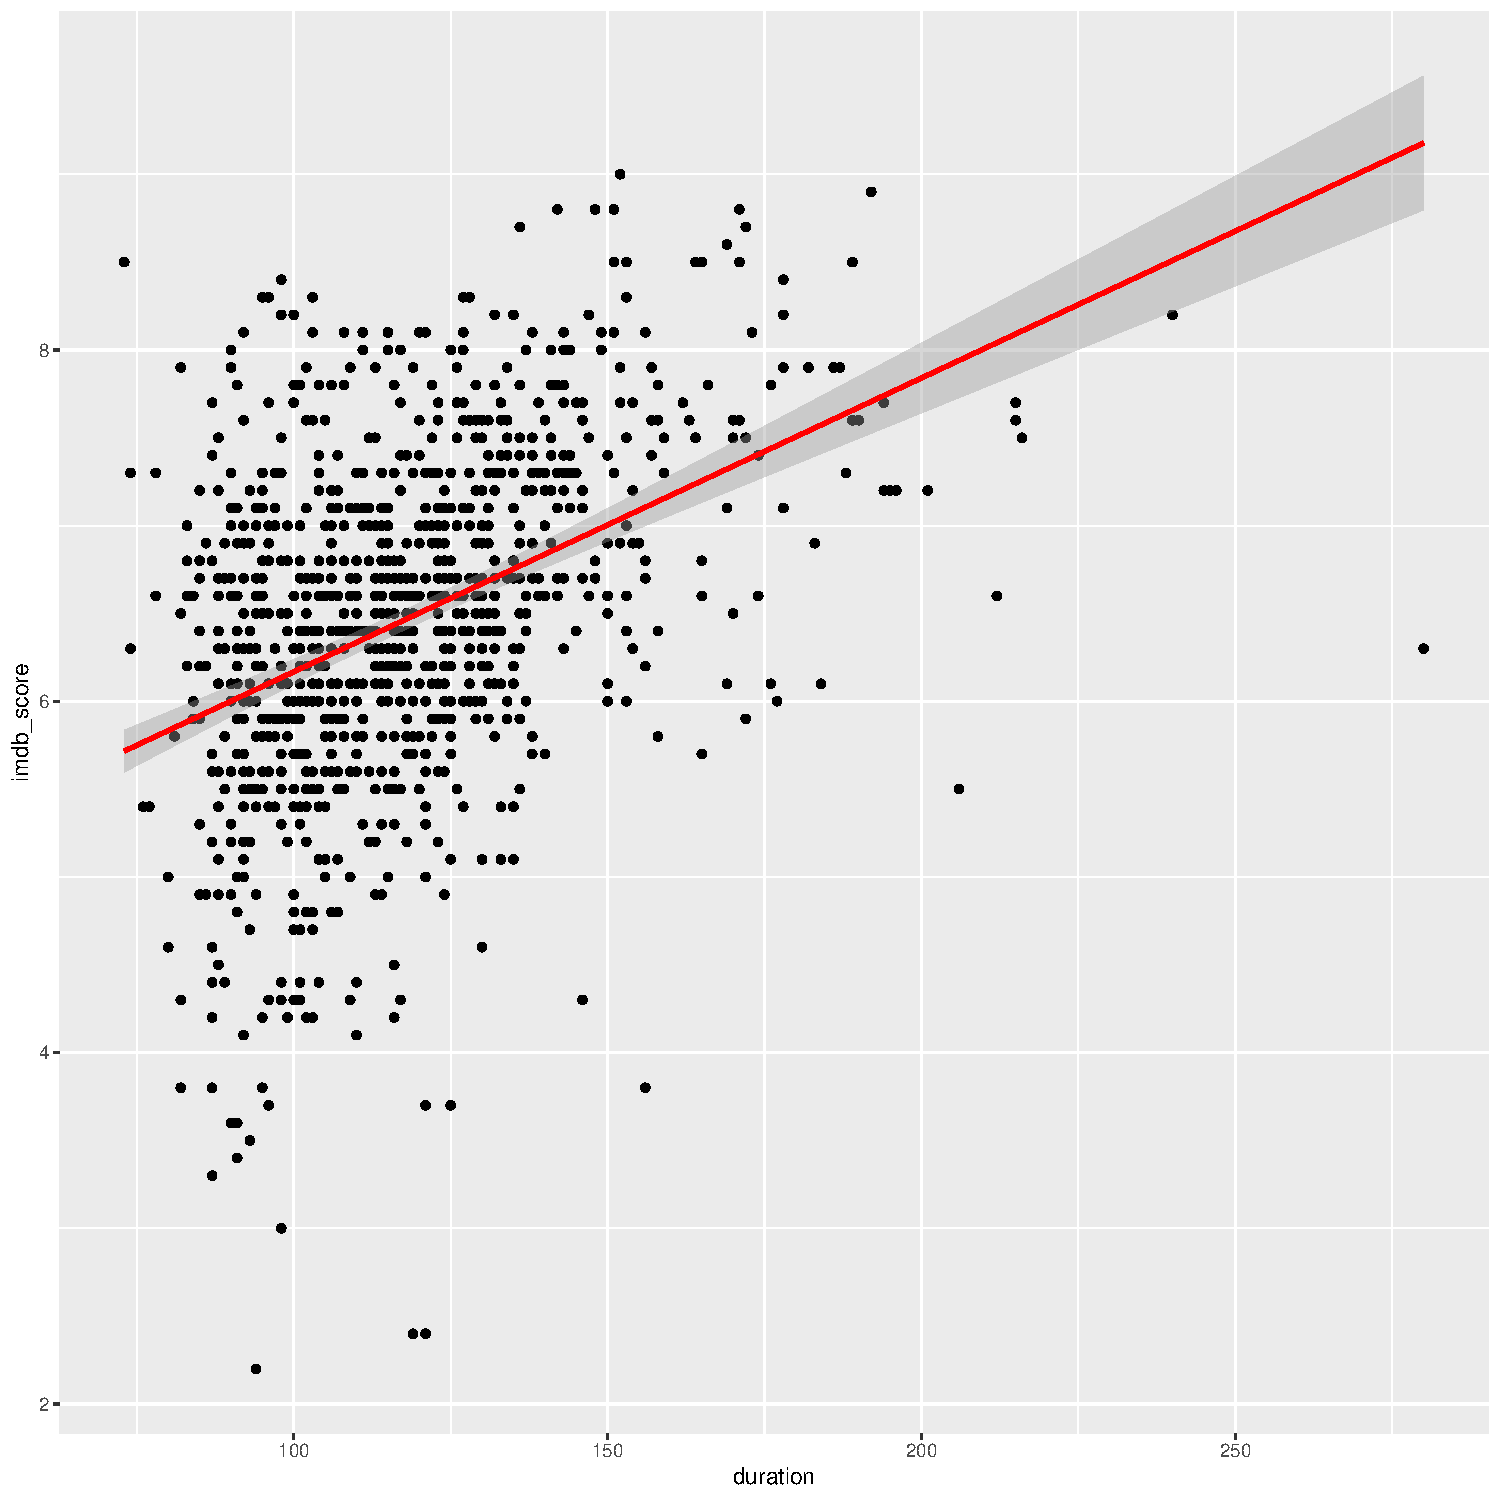
\includegraphics{practica-3-regresion2}

\subsubsection{Árboles de regresión y clasificación}
Ahora realizaremos clasificación tanto de variables cualitativas(árbol de clasificación) como de variables cuantitativas(árbol de regresión), para ello usaremos rpart y tree como métodos para realizar los árboles

Este árbol es un clasificador sobre la variable país (country) de la película, para ello en vez de usar todas las columnas de los datos, usamos solo el nombre de director, la puntuación y el título. Además para indicar de forma explícita que es una clasificación pondremos el method con valor class y las particiones mínimas a 1.
\begin{Schunk}
\begin{Sinput}
> # Arbol de clasificacion (clases)
> clasif.rpart=rpart(country~director_name+imdb_score+title_year,
+                    data=pelis, method="class", minsplit=1)
\end{Sinput}
\end{Schunk}

Como método de visualización hemos usado la biblioteca \textbf{rpart.plot}, que se especializa en mostrar árboles de clase rpart, de los que hemos elegido varias visualizaciones.

\begin{Schunk}
\begin{Sinput}
> rpart.plot(clasif.rpart, type=4)
\end{Sinput}
\end{Schunk}
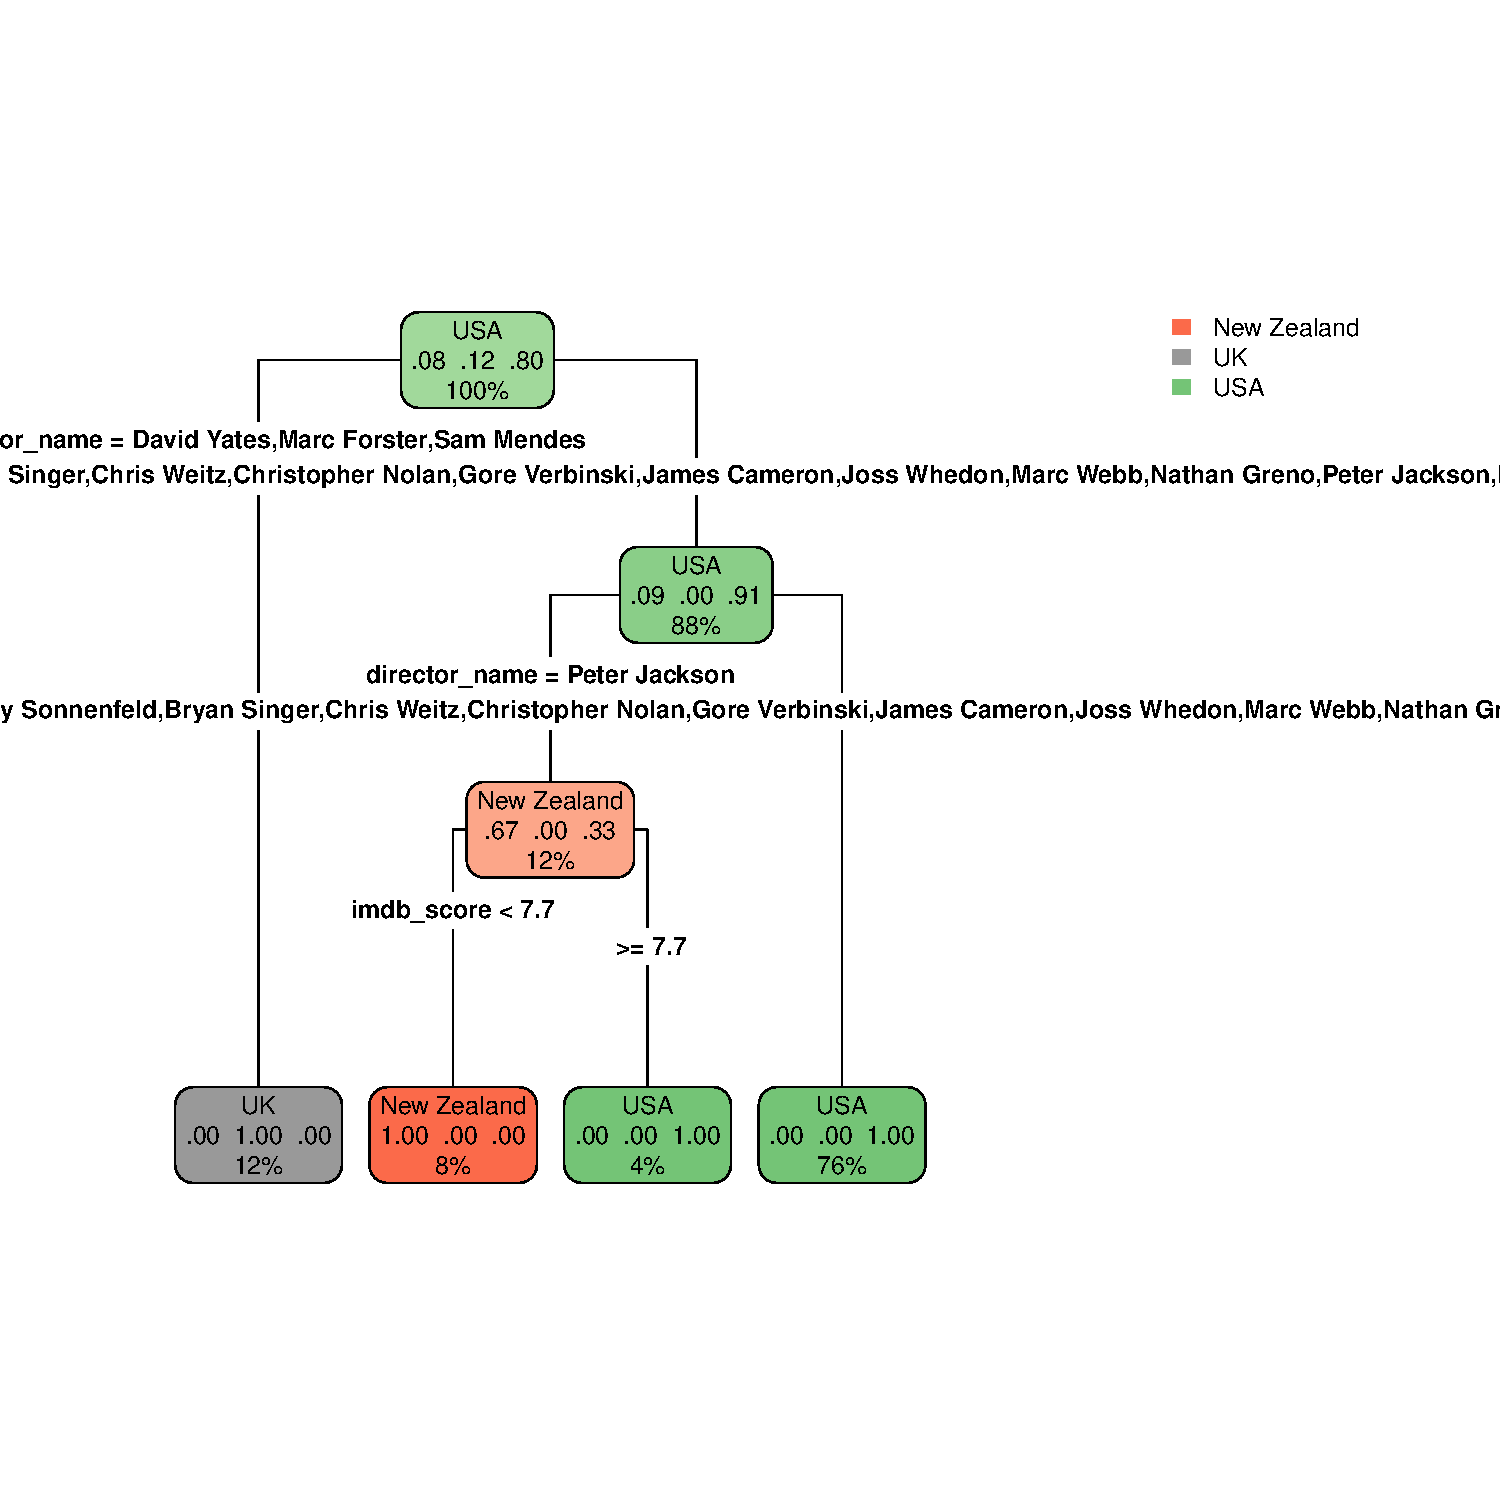
\includegraphics{practica-3-rpart1}
 
 A diferencia del caso anterior, ahora vamos a cambiar parámetros como la optimización, que por defecto se realiza con Gini, ahora la haremos con el método de ganancia de información, que será indicado por los parámetros. También, hemos cambiado las variables a puntuación y año de publicación.
 
\begin{Schunk}
\begin{Sinput}
> # Arbol de clasificacion (clases)
> clasif.rpart2=rpart(country~imdb_score+title_year,data=pelis,
+     method="class",parms = list(split="information"), minsplit=1)
\end{Sinput}
\end{Schunk}

\begin{Schunk}
\begin{Sinput}
> rpart.plot(clasif.rpart2, type=2)
\end{Sinput}
\end{Schunk}
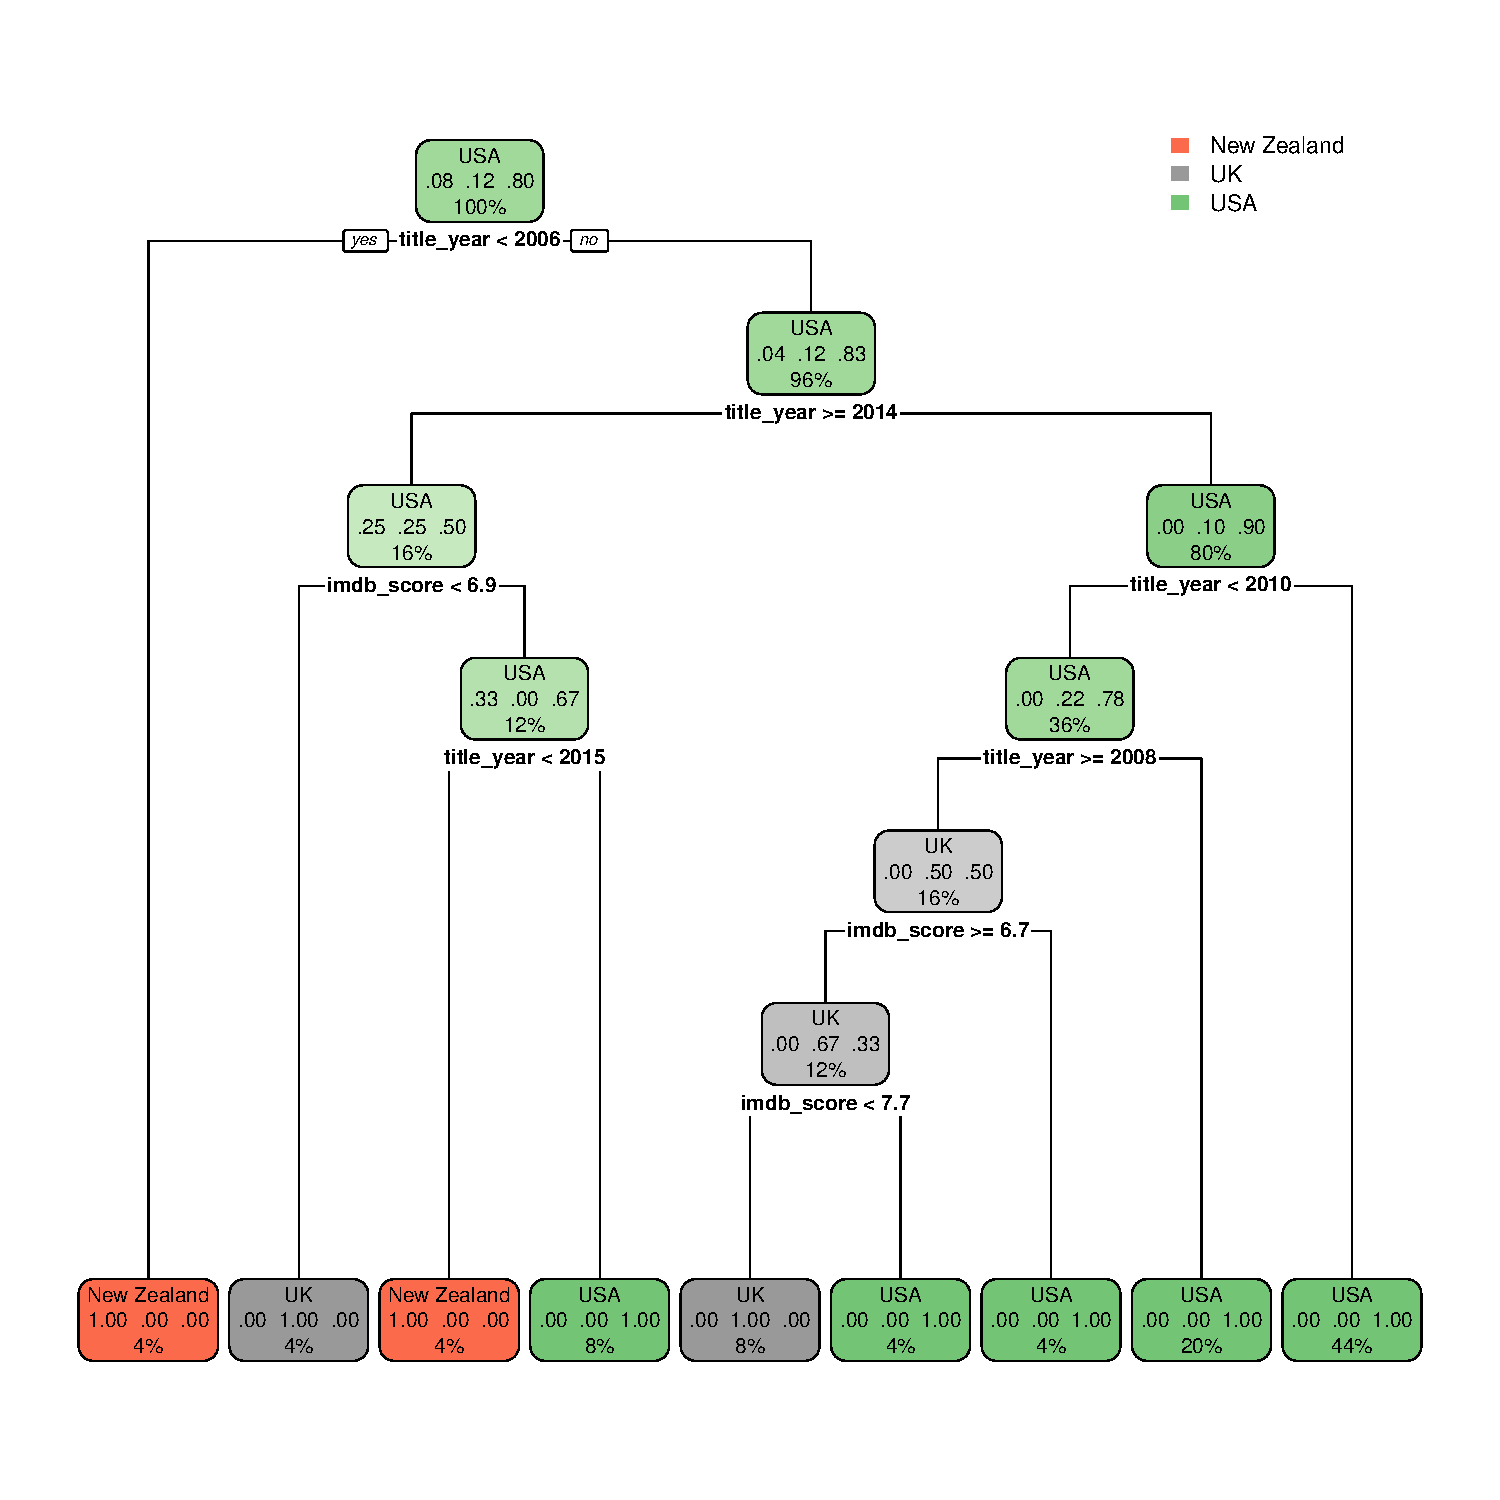
\includegraphics{practica-3-rpart2}

Este árbol será un árbol de regresión, porque trabajará sobre la variable cuantitativa de presupuesto, que será un entero en la divisa del país. Este se obtendrá mediante la fórmula formada por año de publicación, puntuación y número de votos. Como se trata de un árbol de regresión tenemos que cambiar el método a anova.

\begin{Schunk}
\begin{Sinput}
> # Arbol de regresion (numerico)
> anova.rpart=rpart(budget~title_year+imdb_score+num_voted_users
+                   ,data=mil_peliculas, method="anova")
\end{Sinput}
\end{Schunk}

\begin{Schunk}
\begin{Sinput}
> rpart.plot(anova.rpart, type=2)
\end{Sinput}
\end{Schunk}
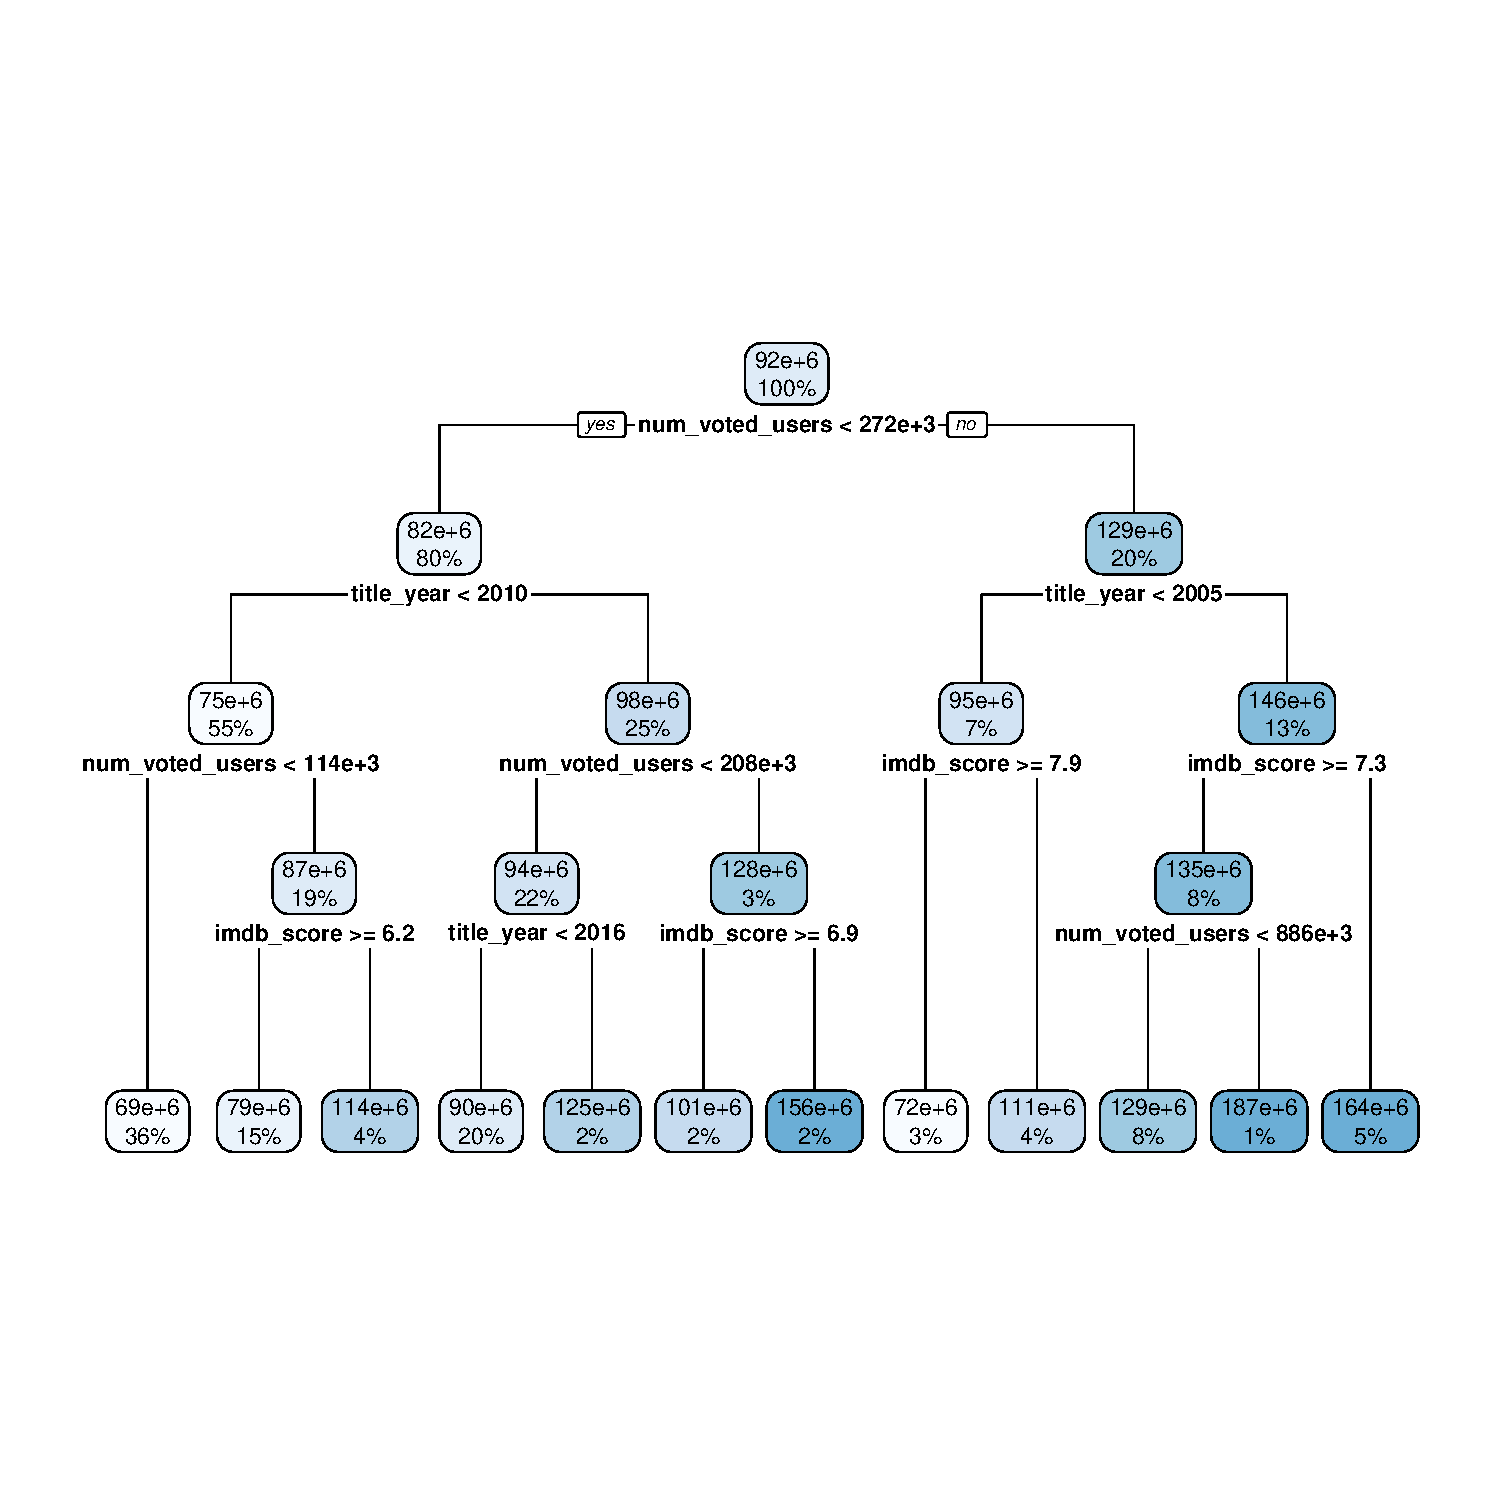
\includegraphics{practica-3-rpart3}

Finalmente, rpart ofrece un módulo para generar reglas que permitan implementar los clasificadores, en este caso mostraremos algunas de las reglas por escrito. Con style="tallw" podremos mostrarlas de forma más clara.

\begin{Schunk}
\begin{Sinput}
> # Reglas que definen los arboles
> reglas.anova <-rpart.rules(anova.rpart,style="tallw")
> head(reglas.anova,2)
\end{Sinput}
\begin{Soutput}
budget is 6.9e+07 when
                  num_voted_users < 114018
                  title_year < 2010

budget is 7.2e+07 when
                  num_voted_users >= 272379
                  title_year < 2005
                  imdb_score >= 7.9
\end{Soutput}
\begin{Sinput}
> rpart.rules(clasif.rpart,style="tallw")
\end{Sinput}
\begin{Soutput}
                        New    UK  USA 
country is New Zealand [1.00  .00  .00] when
                                        director_name is Peter Jackson
                                        imdb_score < 7.7

country is UK          [ .00 1.00  .00] when
                                        director_name is David Yates or Marc Forster or Sam Mendes

country is USA         [ .00  .00 1.00] when
                                        director_name is Peter Jackson
                                        imdb_score >= 7.7

country is USA         [ .00  .00 1.00] when
                                        director_name is Andrew Adamson or Andrew Stanton or Barry Sonnenfeld or Bryan Singer or Chris Weitz or Christopher Nolan or Gore Verbinski or James Cameron or Joss Whedon or Marc Webb or Nathan Greno or Ridley Scott or Rob Marshall or Sam Raimi or Zack Snyder
\end{Soutput}
\end{Schunk}

Esta clasificación es igual a la que realizamos por rpart, con la misma fórmula. Como se puede observar el gráfico del árbol es igual (aunque no en estilo). También como variación se ha cambiado el método de partición a desviación.

\begin{Schunk}
\begin{Sinput}
> # Clasificacion con tree
> clasificacion.tree = tree(budget~title_year+imdb_score+num_voted_users,data=mil_peliculas,split = "deviance")
\end{Sinput}
\end{Schunk}

\begin{Schunk}
\begin{Sinput}
> plot(clasificacion.tree );  
> text(clasificacion.tree , all=TRUE, cex=0.5)
\end{Sinput}
\end{Schunk}
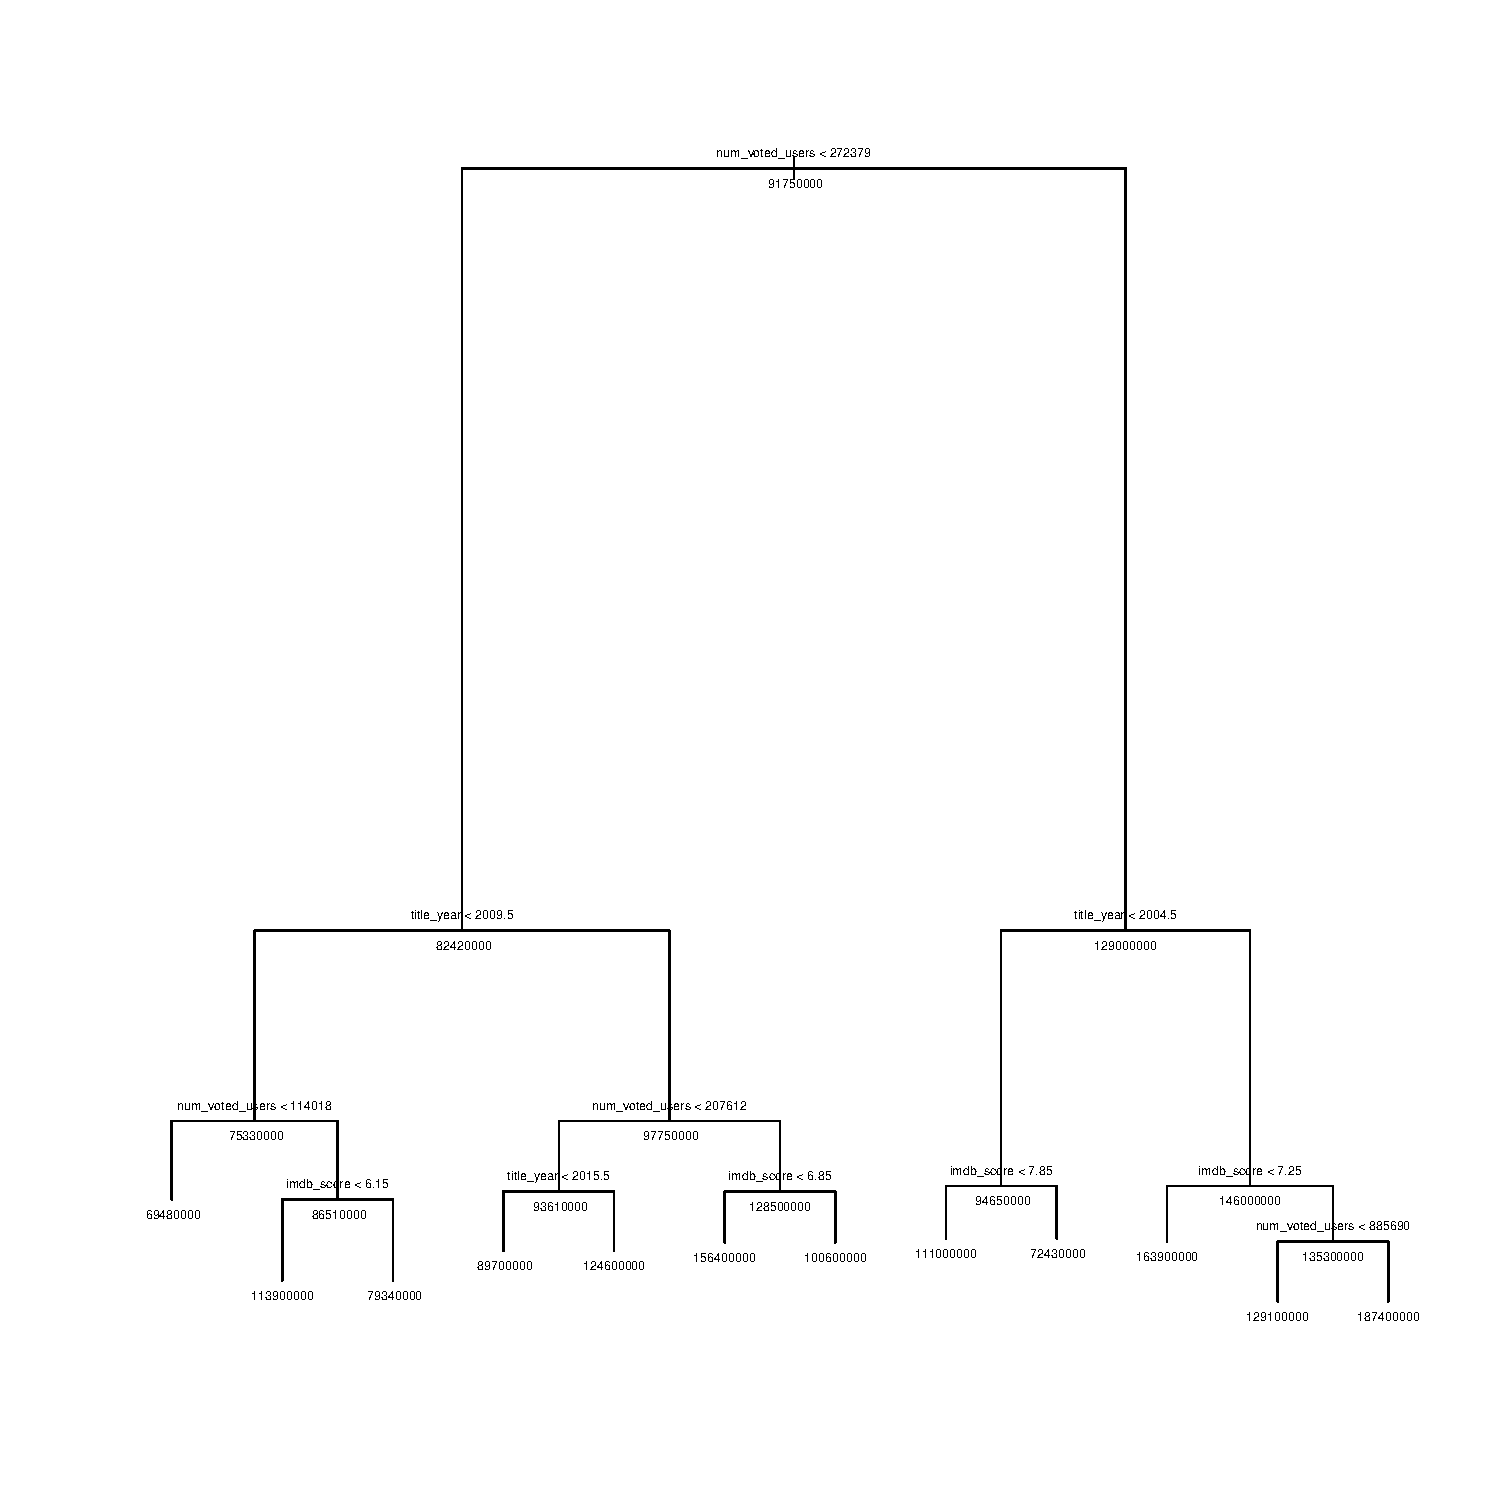
\includegraphics{practica-3-tree}

\subsubsection{Random Forest para clasificación}
Haremos uso de la librería randomForest para otra clasificación de los datos, esta librería implementa el algoritmo de bosque aleatorio de Breiman (random forest) para la clasificación y la regresión. Este algoritmo genera muchos arboles con clasificaciones, cada una con unos votos, el bosque elige la clasificación con más votos teniendo en cuenta todos los árboles del bosque. 

Cada árbol crece de manera que, si el numero de casos en el set de entreno es N, muestra es de N casos al azar pero con "replacement" (el reemplazo) de los datos originales. Esta muestra será el set de entreno para el árbol. Si hay M variables de entrada siendo m variables seleccionadas al azar a partir de M y la mejor división de esta m se usa para dividir el nodo
el valor de m es constante en el crecimiento del bosque, tendremos que m<<M. Cada árbol se crece hasta la extensión más grande posible, no hay poda. 

La tasa de error depende de la correlación entre dos arboles cualquiera en el bosque, cuanta más correlación más ratio de error, y también depende de la fuerza de cada árbol en el bosque, un árbol con poco ratio de error es un clasificador fuerte, a más fuerza de los árboles menos ratio de error en el bosque.
En nuestro ejemplo se hará el entrenamiento con el 70 de los datos y 500 árboles, para mostrarlo en una gráfica que nos dirá la precisión del clasificador en función al número de árboles, que es bastante aceptable, como se podrá ver en el ejemplo de predicción.
\begin{Schunk}
\begin{Sinput}
> set.seed(88)
> # Preparacion datos de entrenamiento
> tamano.total <- nrow(peliculas)
> tamano.entreno <- round(tamano.total*0.7)
> datos.indices <- sample(1:tamano.total , size=tamano.entreno)
> peliculas.entreno <- peliculas[datos.indices,]
> peliculas.test <- peliculas[-datos.indices,]
> # Modelo de random forest
> clasif.randomf = randomForest(imdb_score~title_year+budget+
+                  num_voted_users, data = peliculas.entreno)
\end{Sinput}
\end{Schunk}

\begin{Schunk}
\begin{Sinput}
> plot(clasif.randomf)
\end{Sinput}
\end{Schunk}
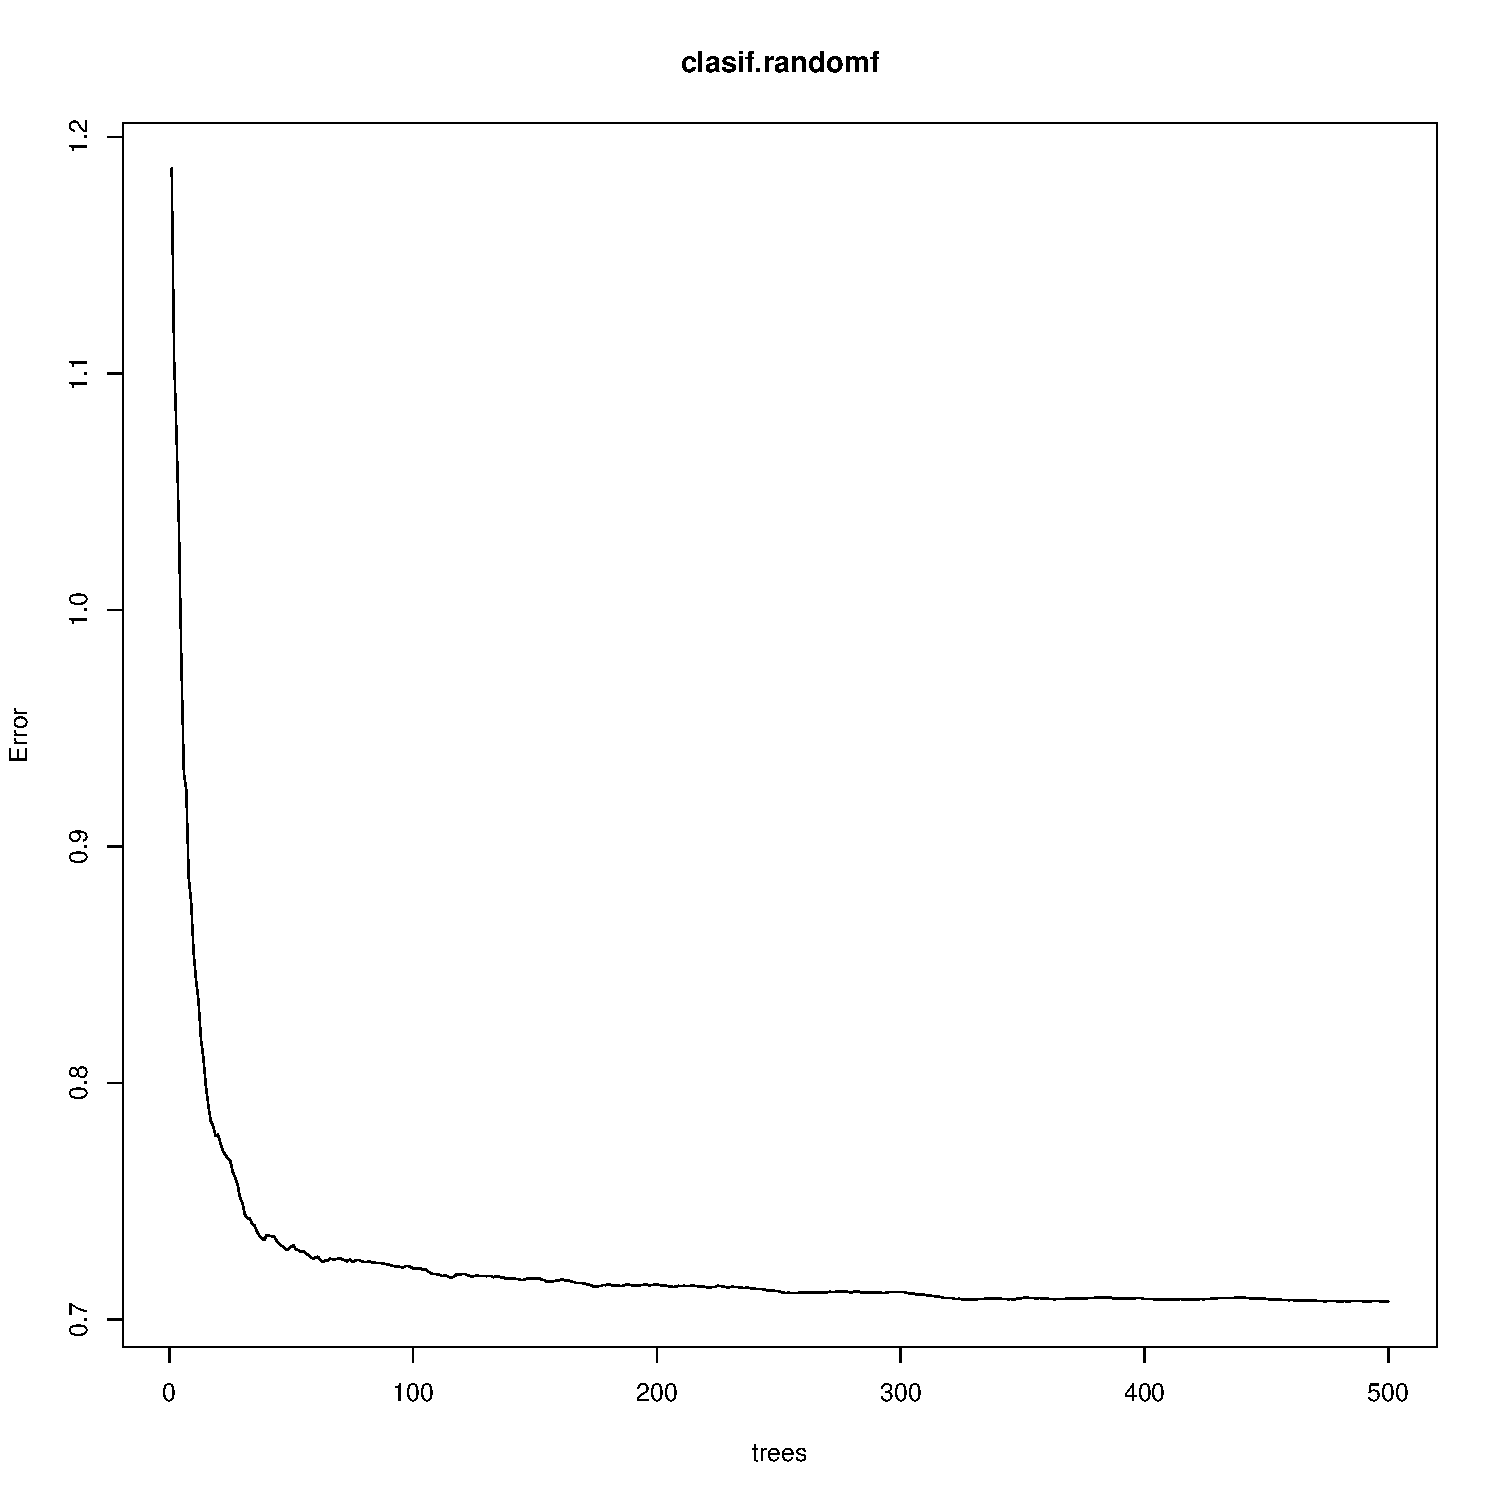
\includegraphics{practica-3-randomf}

\subsubsection{Clasificación bayesiana}
La clasificación bayesiana se basa en la estadística bayesiana, que se basa en la independencia de las características de un objeto, en nuestro caso la película. Entonces usando estas características de forma condicional (una característica puede depender de la anterior) que formará un producto de probabilidades de las características del objeto. Por lo que si una estuviera ausente, esta haría que todo valiese cero.

Implementaremos este tipo de clasificación con la biblioteca bayesTrees y usaremos el método bart. Este recibe los datos a entrenar y targets que en este caso son número de votos y puntuaciones. Además si quisieramos podríamos añadir datos para hacer el test con el mismo método.
\begin{Schunk}
\begin{Sinput}
> set.seed(99)
> clasif.bart <- bart(pelis["num_voted_users"],as.double(pelis$imdb_score))
\end{Sinput}
\begin{Soutput}
Running BART with numeric y

number of trees: 200
Prior:
	k: 2.000000
	degrees of freedom in sigma prior: 3
	quantile in sigma prior: 0.900000
	power and base for tree prior: 2.000000 0.950000
	use quantiles for rule cut points: 0
data:
	number of training observations: 25
	number of test observations: 0
	number of explanatory variables: 1


Cutoff rules c in x<=c vs x>c
Number of cutoffs: (var: number of possible c):
(1: 100) 


Running mcmc loop:
iteration: 100 (of 1100)
iteration: 200 (of 1100)
iteration: 300 (of 1100)
iteration: 400 (of 1100)
iteration: 500 (of 1100)
iteration: 600 (of 1100)
iteration: 700 (of 1100)
iteration: 800 (of 1100)
iteration: 900 (of 1100)
iteration: 1000 (of 1100)
iteration: 1100 (of 1100)
time for loop: 1

Tree sizes, last iteration:
2 2 2 3 2 2 2 2 3 1 2 2 2 2 3 3 2 3 4 3 
2 2 2 3 2 2 2 3 2 2 2 2 3 4 2 2 2 4 2 2 
3 2 2 2 2 2 3 2 2 2 2 3 2 2 2 3 1 2 2 2 
2 2 3 2 2 1 4 2 3 3 2 2 4 2 2 2 2 3 2 2 
2 2 2 1 2 3 2 3 4 3 2 2 1 2 3 2 2 2 2 3 
1 3 3 2 2 2 2 2 4 3 2 2 2 2 2 1 2 3 3 2 
2 1 2 3 3 3 3 2 2 1 2 3 2 2 3 3 2 2 2 2 
2 2 2 1 2 2 2 2 2 2 4 2 3 2 2 2 2 2 2 3 
2 2 2 2 2 3 3 3 2 3 2 3 2 3 2 2 2 2 2 2 
2 2 2 2 2 2 2 3 2 3 2 2 3 2 2 2 2 2 2 3 
Variable Usage, last iteration (var:count):
(1: 252) 
DONE BART 11-2-2014
\end{Soutput}
\end{Schunk}

El resultado son dos gráficas que muestran los datos, en la izquierda la sigma de cada objeto, y a la derecha las puntuaciones en las que clasificará junto a sus desviaciones.

\begin{Schunk}
\begin{Sinput}
> plot(clasif.bart)
\end{Sinput}
\end{Schunk}
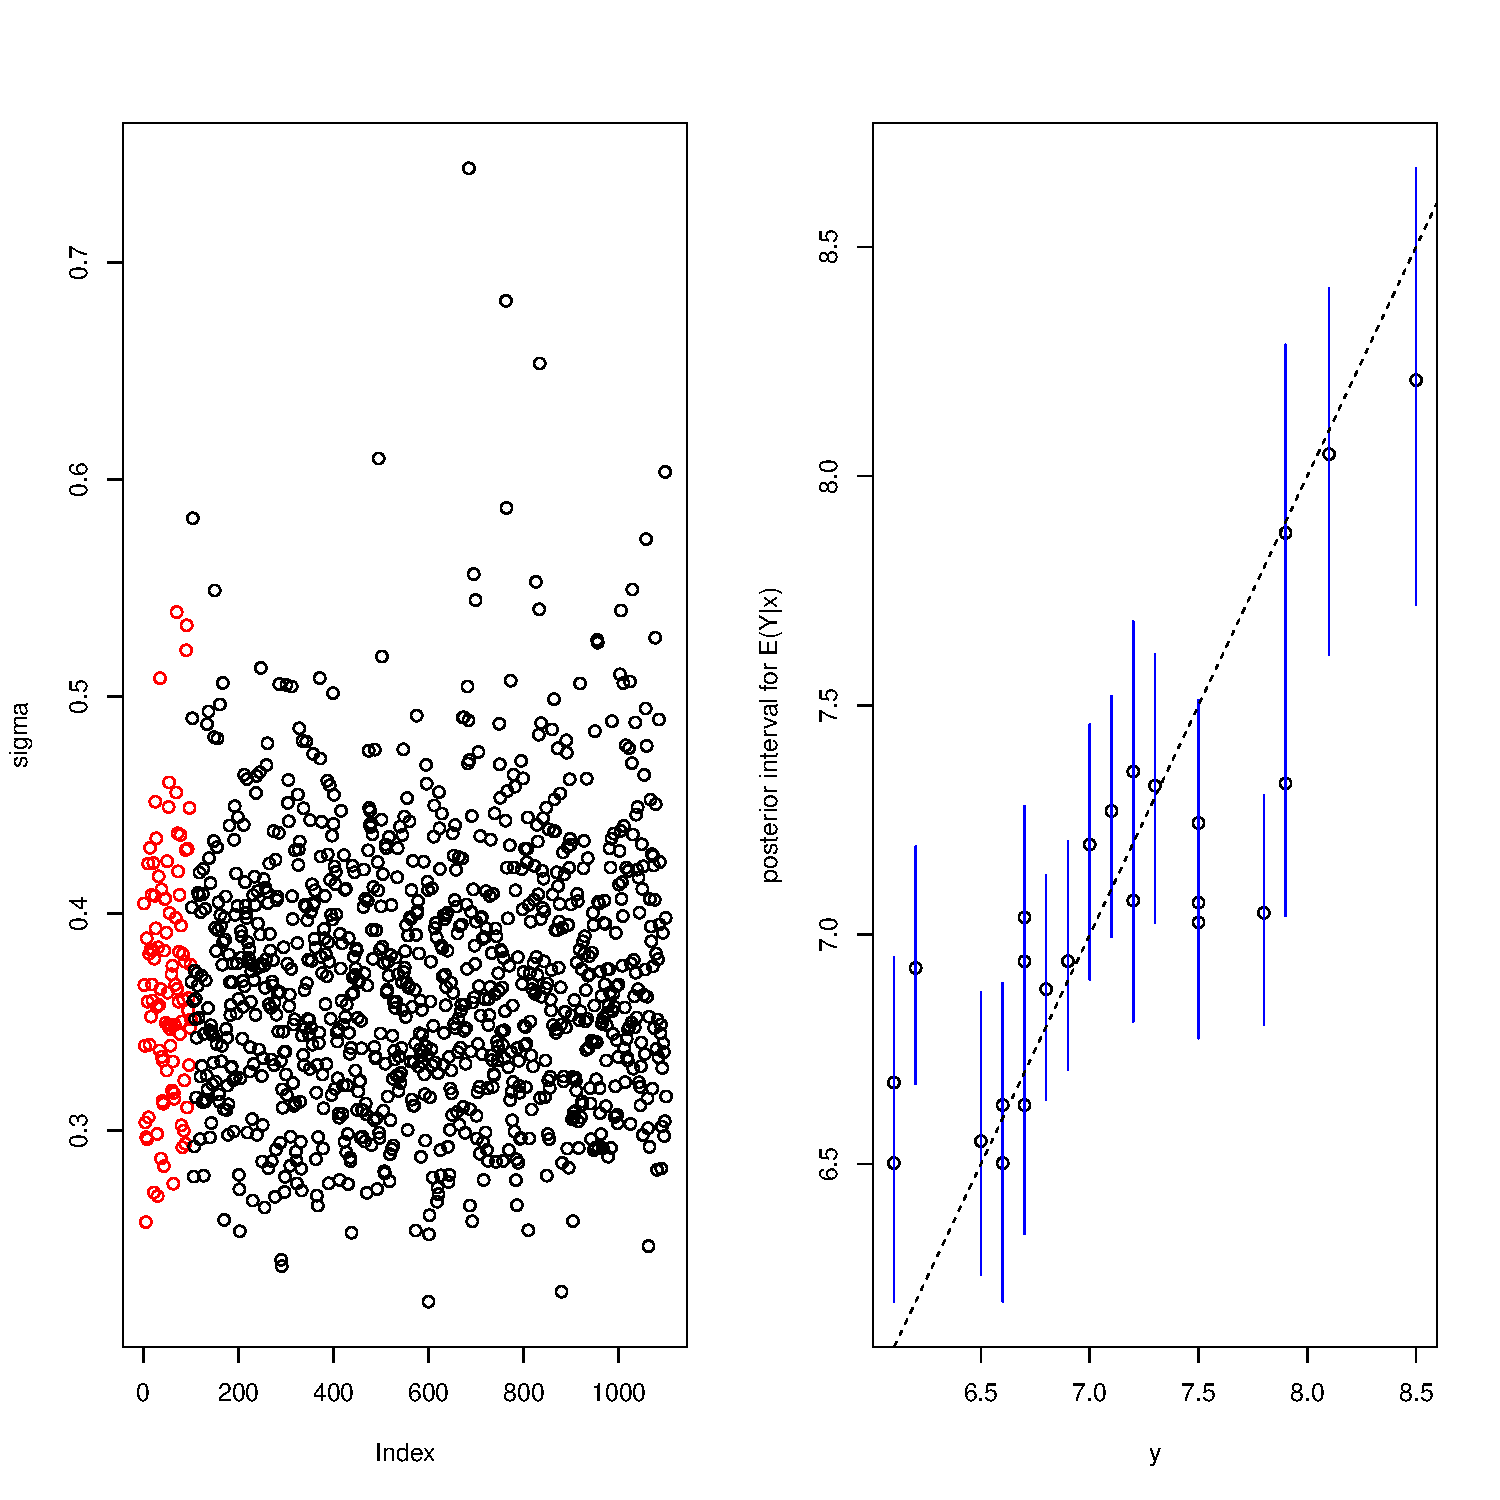
\includegraphics{practica-3-bart}

\subsubsection{Predicción de datos con los modelos}
Para finalizar la práctica vamos a usar los modelos creados anteriormente para realizar predicciones de clasificación, dentro lo posible. Como herramienta usaremos el método predict que implementan rpart y randomForest, para realizar las predicciones.

En los árboles de clasificación, se pueden usar los tipos prob, que muestra la probabilidad de cada valor cualitativo de la variable y class que muestra las distintas clases a las que se llega.

En los árboles de regresión, solo se puede aplicar matrix y vector, ambos devuelven la respuesta media al objeto a clasificar, en este caso solo haremos vector, al cambiar sólo la forma de representación.

La predicción con randomForest funciona de forma similar, aunque no es necesario indicar el tipo, pero si queremos generar todas las decisiones de los árboles lo indicaremos con predict.all.
\begin{Schunk}
\begin{Sinput}
> # Predicciones
> # Probabilidades y factores predecidos
> head(predict(clasif.rpart, type = "prob"),10)
\end{Sinput}
\begin{Soutput}
   New Zealand UK USA
1            0  0   1
2            0  0   1
3            0  1   0
4            0  0   1
6            0  0   1
7            0  0   1
8            0  0   1
9            0  0   1
10           0  1   0
11           0  0   1
\end{Soutput}
\begin{Sinput}
> predict(clasif.rpart, type = "class")
\end{Sinput}
\begin{Soutput}
          1           2           3           4           6           7 
        USA         USA          UK         USA         USA         USA 
          8           9          10          11          12          13 
        USA         USA          UK         USA         USA          UK 
         14          15          16          17          18          19 
        USA         USA         USA         USA         USA         USA 
         20          21          22          23          24          25 
        USA New Zealand         USA         USA         USA         USA 
         26 
New Zealand 
Levels: New Zealand UK USA
\end{Soutput}
\begin{Sinput}
> # Respuesta media para regresion
> predict(anova.rpart,peliculas[2555,], type = "vector")
\end{Sinput}
\begin{Soutput}
    2824 
89698990 
\end{Soutput}
\begin{Sinput}
> predict(anova.rpart,peliculas[1268,], type = "vector")
\end{Sinput}
\begin{Soutput}
    1339 
69475376 
\end{Soutput}
\begin{Sinput}
> predict(anova.rpart,peliculas[1150,], type = "vector")
\end{Sinput}
\begin{Soutput}
     1214 
129090667 
\end{Soutput}
\begin{Sinput}
> # Prediccion con random forest
> peliculas.test[2,]
\end{Sinput}
\begin{Soutput}
   director_name num_critic_for_reviews duration     actor_2_name     gross
10   David Yates                    375      153 Daniel Radcliffe 301956980
                             genres actor_1_name
10 Adventure|Family|Fantasy|Mystery Alan Rickman
                               movie_title num_voted_users language country
10 Harry Potter and the Half-Blood Prince           321795  English      UK
    budget title_year imdb_score
10 2.5e+08       2009        7.5
\end{Soutput}
\begin{Sinput}
> prediccion.rf<-predict(clasif.randomf, peliculas.test[3,], predict.all=TRUE)
> prediccion.rf[[1]]
\end{Sinput}
\begin{Soutput}
      11 
7.549481 
\end{Soutput}
\end{Schunk}

Como podemos ver los resultados en las predicciones en las que hemos introducido los datos son coherentes como se ve con las puntuaciones con el random forest o con los prespuestos, estas últimas un poco menos coherentes.
\end{document}
